This chapter will go into the results of the simulation and the validation of the success of the chosen approach. Two metrics have been chosen to analyze simulation runs:

\begin{enumerate}
	\item The duration of the simulation in seconds from the first agent being spawned until the last agent arrives at his target.
	\item The the number of active agents in the network measured at a fixed time interval (5 minutes).
\end{enumerate}

The street network used is the one visible in \autoref{otfvis}. The main start point for agent is the top of the highway, additional smaller inputs are placed around the border of the network. The routes are defined in a way, that most of the agents must drive over the main street that comes from the highway and goes to the right to the large roundabout, which is where the main ''hotspots`` are supposed to form. The rest of the routes are distributed fairly evenly over the rest of the network.

The population size was set to 10,000 agents. These agents try to reach their destination links within a time frame of about 16.5 hours (60,000 seconds).

For reference, a simple fixed-cycle signal controller is used, that has a configurable constant phase duration and cycles through the phases in a random but stable order. This represents a situation with unoptimized static signal control systems. In \autoref{cycle_based_results} the simulation duration for this signal controller with different phase durations can be seen. The simulations took all around 70 hours (three days). The optimal phase duration for the given scenario based on these tests is somewhere between two and three minutes. For further tests and comparisons, a duration of two minutes is thus used.

\begin{figure}
	\centering	
	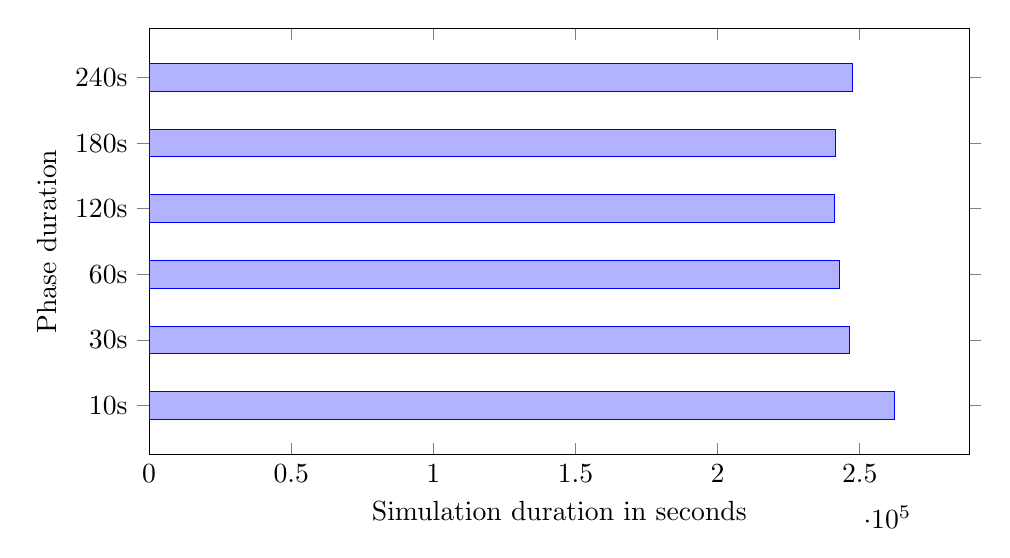
\begin{tikzpicture}
	\begin{axis}[
		xbar,
		xmin=0,
		width=12cm,
		height=7cm,
		enlarge y limits=0.15,
		xlabel={Simulation duration in seconds},
		ylabel={Phase duration},
		symbolic y coords={10s,30s,60s,120s,180s,240s},
		ytick=data,
		nodes near coords align={horizontal},
	]
	\addplot coordinates {(262385,10s) (246490,30s) (242953,60s) (240975,120s) (241523,180s) (247402,240s)};
	\end{axis}
	\end{tikzpicture}
	\label{cycle_based_results}
	\caption{Simulation durations for the fixed cycle signal controller.}
\end{figure}

The fixed-cycle signal controller is compared to the stress-based signal controller, using a priority queue like approach instead of cycles (see \autoref{trafficLightController} for more details). The stress functions are selected from a small set of defined functions to show the differences they can make.

The following four functions ($\mathbb{R}^2 \mapsto \mathbb{R}$) have been selected, including the function shown in \autoref{stress_func_plot}, here as function $h$:

\begin{enumerate}
	\item $f(n, t) = w_n n + w_tt$
	\item $g(n, t) = \frac{w_n n^2}{2} + \frac{w_t t^2}{2}$
	\item $h(n, t) = (n + t)(n + c)$ (see \autoref{proposed_stress})
	\item $i(n, t) = n$
\end{enumerate}

The functions $f$ and $g$ where added as a comparison due to their simplicity and balanced influence of car count and the red time. The function $i$ has been added as a variant that does not include the time aspect to verify the statement mentioned in \autoref{stress_prio} about the importance of it. The constant weights for the car count and red time (functions $f$ and $g$) have been chosen as $w_n = 1$ and $w_t = 1.1$ for the following test, to give a slightly bigger influence to the red time. The constant $c$ (function $h$) has been chosen as $c = 0.1$ to allow stress growth even when the car count is zero, only based on the time.

The phase duration has been calculated with ten seconds per waiting vehicles with a minimum of ten seconds and a maximum of 100 seconds.

\begin{figure}
\centering	
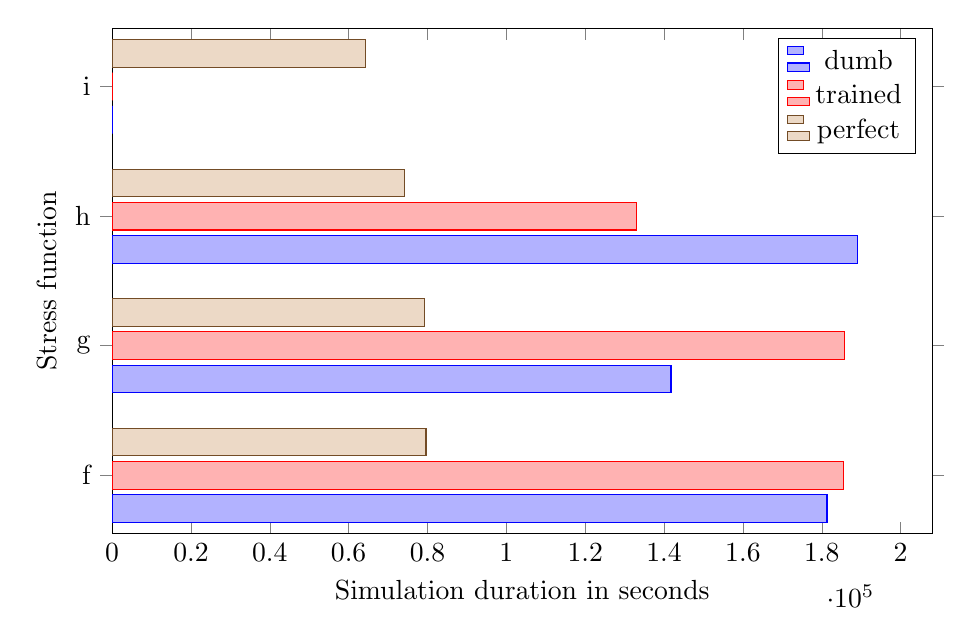
\begin{tikzpicture}
\begin{axis}[
	xbar,
	xmin=0,
	width=12cm,
	height=8cm,
	enlarge y limits=0.15,
	xlabel={Simulation duration in seconds},
	ylabel={Stress function},
	symbolic y coords={f,g,h,i},
	ytick=data,
	nodes near coords align={horizontal},
]
\addplot coordinates {(0,i) (189149,h) (141760,g) (181329,f)};
\addplot coordinates {(0,i) (132996,h) (185709,g) (185400,f)};
\addplot coordinates {(64249,i) (74127,h) (79132,g) (79625,f)};
\legend{dumb,trained,perfect}
\end{axis}
\end{tikzpicture}
\label{stress_based_results}
\caption{Simulation durations for the stress based signal controller.}
\end{figure}

Looking at \autoref{stress_based_results}, the first thing to notice, is that the function $i$ has only one value compared to three like the other functions have. All four stress function were tested under three conditions:

\begin{enumerate}
	\item With an untrained prediction network, so predictions are basically random.
	\item With a trained prediction network.
	\item With perfect (always correct) predictions.
\end{enumerate}

This shows two things: First what influence the prediction quality has on the switching performance (untrained being the worst case, perfect predictions the best case) and secondly how well the learning and the prediction perform.

This diagram directly confirms the importance of the time factor as mentioned in \autoref{stress_prio}, as the function $i$ caused to simulation to get stuck sooner or later in all tests. Errors in the prediction can result in stress at signals where no vehicles are waiting, while signals that have cars might get less stress or none at all. In these situations, the traffic at that location is stuck forever. In reality, people would eventually start to ignore the red signal or turn around and use a different route, but the simulation agents will not do this. While this function can fail in these situations, in a perfect world it would perform best.

\begin{figure}[ht!]
	\centering
	\begin{tikzpicture}
	\begin{axis}[
		width=15cm,
		height=8cm,
		xmin=0,
		ymin=0,
		xlabel={Time in seconds},
		ylabel={Agents in the Network}
	]
	\addplot[mark=none,draw=red,thick] table [col sep=comma] {data/agents/cycle.csv};
	\addplot[mark=none,draw=blue,thick] table [col sep=comma] {data/agents/stress/dumb/sumnquadtlin.csv};
	\addplot[mark=none,draw=black,thick] table [col sep=comma] {data/agents/stress/dumb/sumnlintlin.csv};
	\addplot[mark=none,draw=purple,thick] table [col sep=comma] {data/agents/stress/dumb/sumnlinintegtlininteg.csv};
	\addplot[mark=none,draw=green,thick] table [col sep=comma] {data/agents/stress/dumb/nlin.csv};
	\legend{Cycle Controller, {h(n, t)}, {f(n, t)}, {g(n, t)}, {i(n, t)}}
	\end{axis}
	\end{tikzpicture}
	\label{agent_statistic_dumb}
	\caption{Agents living per time unit without previous learning.}
\end{figure}


In a perfect world without prediction errors, all functions perform comparably well with only a few hours difference and all under 24 hours. The more relevant results are those from more realistic situations where prediction errors occur. Here the simulation takes roughly twice as long no matter if the prediction network was trained or not. Only function $h$ showed an improvement after training the prediction. While all stress-based tests are significantly faster then cycle-based tests, these results show already, that the training of the prediction network is not yet good enough, to produce a significantly better result than an untrained network.
The second metric, the number of active/living simulation agents over time, show not only how long the simulation was running, but also how well the network was keeping up with the demand. All four functions and the cycle-base controller as a reference, have each been graphed without training the network, with a trained network and finally with 100\% accurate predictions.

In \autoref{agent_statistic_dumb} the graphs for the test with the untrained network can be seen. The graph of the function $i$ (green line) clearly shows how bad this function performs when the predictions are wrong. The graphs all peek at 60,000 seconds (about 16.5 hours) when the last agent gets spawned. That is also the time, when the traffic jams are the biggest, the largest being at the central intersecting on the main street and where the highway enters the main street. The other stress functions perform similar to the cycle based controller with a similarly high peek around 5,000 agents, but the number of agents decreases more quickly. The $i$ function however keeps almost the entire population inside the network and only loses less than 2000 agents until it peeks and then stays stable.

\begin{figure}[ht!]
	\centering
	\begin{tikzpicture}
	\begin{axis}[
		width=15cm,
		height=8cm,
		xmin=0,
		ymin=0,
		xlabel={Time in seconds},
		ylabel={Agents in the Network}
	]
	\addplot[mark=none,draw=red,thick] table [col sep=comma] {data/agents/cycle.csv};
	\addplot[mark=none,draw=blue,thick] table [col sep=comma] {data/agents/stress/learned/sumnquadtlin.csv};
	\addplot[mark=none,draw=black,thick] table [col sep=comma] {data/agents/stress/learned/sumnlintlin.csv};
	\addplot[mark=none,draw=purple,thick] table [col sep=comma] {data/agents/stress/learned/sumnlinintegtlininteg.csv};
	\addplot[mark=none,draw=green,thick] table [col sep=comma] {data/agents/stress/learned/nlin.csv};
	\legend{Cycle Controller, {h(n, t)}, {f(n, t)}, {g(n, t)}, {i(n, t)}}
	\end{axis}
	\end{tikzpicture}
	\label{agent_statistic_learned}
	\caption{Agents living per time unit with previous learning.}
\end{figure}

The second diagram, \autoref{agent_statistic_learned}, more clearly shows the improvement when training the prediction network. Function $i$ peaks at about 8,000 agents, then loses a few hundred agents before becoming stable again. While the problem is still there, an improvement is already visible. A real improvement can be seen with function $h$, as it peaks at only about 3000 agents and only after another 17 to 18 hours all agents are gone. That is a good improvement and almost 50\% better than the cycle-based controller both in simulation duration and peak agent count. Functions $f$ and $g$ performed both about the same as without any training.

Finally under optimal conditions the results are, which is to be expected, much better. The functions $f$ and $g$ have the highest peak in this scenario with still over 2,000 agents at the same time on the streets, $h$ is only slightly better. The $i$ function's graph is interesting, because there is almost no buildup of agents in the network and it peaks below 1,000 agents which are gone just about an hour later.

The last two diagrams show that with good predictions, less weight on the time aspects yields better results. No time aspect however will lead to problems in the real world. 

\begin{figure}[bt!]
	\centering
	\begin{tikzpicture}
	\begin{axis}[
		width=15cm,
		height=8cm,
		xmin=0,
		ymin=0,
		xlabel={Time in seconds},
		ylabel={Agents in the Network}
	]
	\addplot[mark=none,draw=red,thick] table [col sep=comma] {data/agents/cycle.csv};
	\addplot[mark=none,draw=blue,thick] table [col sep=comma] {data/agents/stress/perfect/sumnquadtlin.csv};
	\addplot[mark=none,draw=black,thick] table [col sep=comma] {data/agents/stress/perfect/sumnlintlin.csv};
	\addplot[mark=none,draw=purple,thick] table [col sep=comma] {data/agents/stress/perfect/sumnlinintegtlininteg.csv};
	\addplot[mark=none,draw=green,thick] table [col sep=comma] {data/agents/stress/perfect/nlin.csv};
	\legend{Cycle Controller, {h(n, t)}, {f(n, t)}, {g(n, t)}, {i(n, t)}}
	\end{axis}
	\end{tikzpicture}
	\label{agent_statistic_perfect}
	\caption{Agents living per time unit with perfect predictions.}
\end{figure}
